\documentclass[a4paper, titlepage]{article}

\usepackage[utf8]{inputenc}
\usepackage[ngerman]{babel}
\usepackage[T1]{fontenc}
\usepackage{lmodern}

\usepackage{float}

\usepackage{graphicx}
\usepackage{tabularx}

\newcolumntype{b}{X}
\newcolumntype{s}{>{\hsize=.5\hsize}X}
\newcommand{\heading}[1]{\multicolumn{1}{c}{#1}}

\title{Strategiepapier Alte Moschti}
\author{Sascha Huber, Aaron Stampa, Damien Flury}
\date{07. September 2018}

\begin{document}

\maketitle

\tableofcontents
\newpage

\section{Anspruchsgruppen}
\subsection{Kundinnen und Kunden}
\begin{itemize}
  \item Günstige Eintrittspreise
  \item Essen günstig, Getränke ein wenig teurer
  \item Newcomer
  \item Exklusive, interessante Musik
  \item Kunterbuntes Musikangebot
\end{itemize}
\subsection{Eigenkaptialgeber/Eigentümer}
Mit dem Gewinn möchten wir die Dienstleistungen verbessern, d.h. weitere Musiker engangieren,
Werbekampagnen starten, etc. Als Genossenschaft möchten wir unser privates Vermögen von der
alten Moschti trennen und somit unsere Sicherheit gewähren. Zunächst streben wir ein nicht gewinnorientertes
Geschäftsmodell an, später werden wir eine Migration zu einer Aktiengesellschaft in Betracht ziehen.
\subsection{Fremdkapitalgeber}
Gut platzierte, sichtbare Werbung für Fremdkapitalgeber, die Moschti läuft zu regelmässigen Zeiten.
\subsection{Mitarbeiternde}
Fairer Lohn. Gute Arbeitsatmosphäre. Gratiseintritt zur Moschti und kostenlose Getränke.
\subsection{Lieferanten}
Langfristige Beziehungen, pünktliche Bezahlung, gut platzierte Werbung für Lieferanten.
\subsection{Institutionen}
Umweltgerechtes Verhalten, Müll trennen, gute Arbeitsbedingungen, Sponsoring
\subsection{Staat}
Steuereinnahmen, Einhalten von Gesetzen, langfristige Arbeitsstellen.
\subsection{Konkurrenz}
Fairer Wettkampf, gegenseitige Unterstützung

\section{Umweltsphären}
\subsection{Ökonomische Umweltsphäre}
Ökonomische Risiken sind plötzliche Wirtschaftskrisen, Inflation, sinkende Arbeitslöhne, 
konstante Wirtschaftslage.
\subsection{Technologische Umweltsphäre}
Neue Techno-Partys in der Umgebung.
\subsection{Ökologische Umweltsphäre}
Verhinderung der Zufahrt zur Moschti aufgrund Strassensperren, etc.
\subsection{Soziale Umweltsphäre}
Rauchverbot in der Moschti, erlaubt ausserhalb. 
\section{Zentrale Werte}
\begin{itemize}
  \item Unterstützung unbekannter Musiker
  \item Für die Gesellschaft
  \item Musik für Jung und Alt
  \item Schutz der Umwelt
\end{itemize}
\section{Vision}
Möglichst viele Menschen mit der Moschti erreichen, unterhalten und die Gewinne wieder in die Moschti investieren. 
\section{Öffentliches Leitbild}
Wir sind daran interessiert, unsere Leitsungen stets zu verbessern und somit allen Kunden gerecht zu werden.
\section{SWOT-Analyse und Unternehmensstrategie}
\begin{figure}[H]
  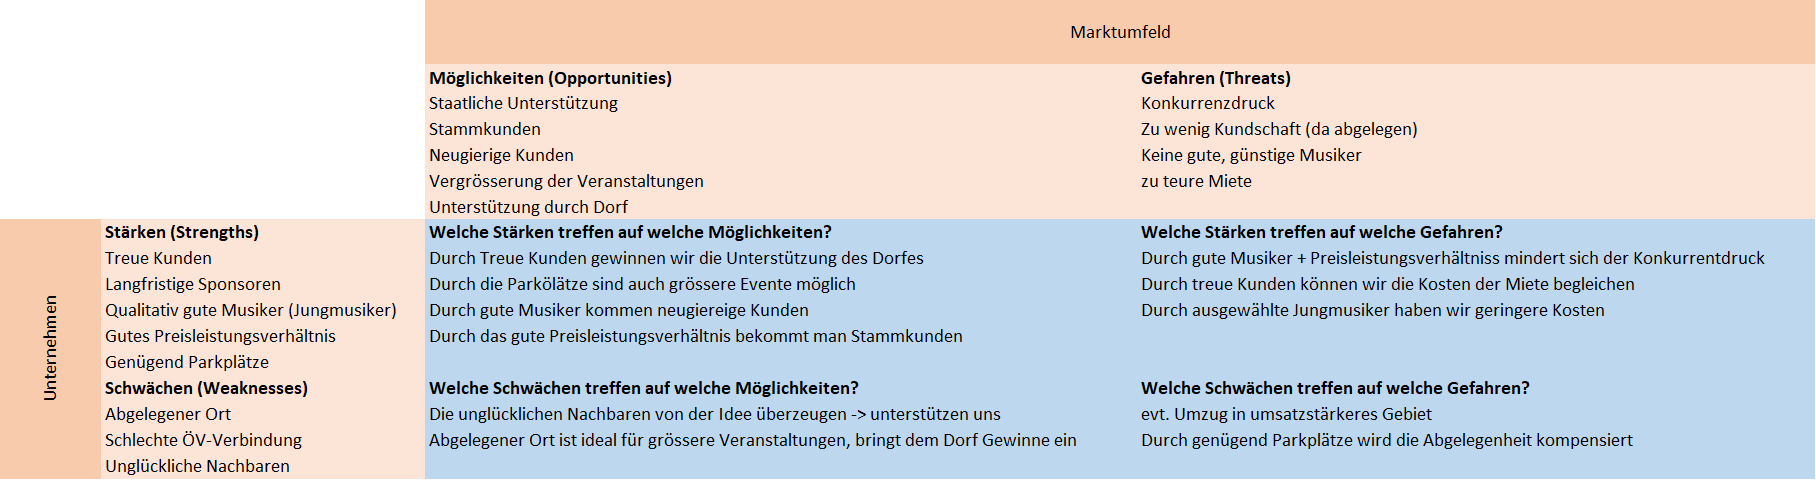
\includegraphics[width=\textwidth]{swot_analysis}
  \caption{SWOT-Analyse}
\end{figure}


\section{Wettbewerbsstrategie}
Wir setzen auf die Gesamtmarktstrategie, da wir Events in sämtliche Richtungen anbieten und somit alle Bedürfnisse versuchen abzudecken.

\section{Nutzwerkanalyse}
Durch die Nutzwerkanalyse wurde ersichtlich, dass der Standort im berner Dorf am geignetsten ist. 
Dies, da die Mietpreise günstig sind und die Kunden nur bedingt spontan entscheiden können, da man manchmal Tickets für ein Mosti-Event braucht.
Somit entscheiden wir in dem berner Dorf zu bleiben und zu hoffen, dass wir die Bevölkerung von unserer Sache überzeugen können.

\begin{figure}[h]
  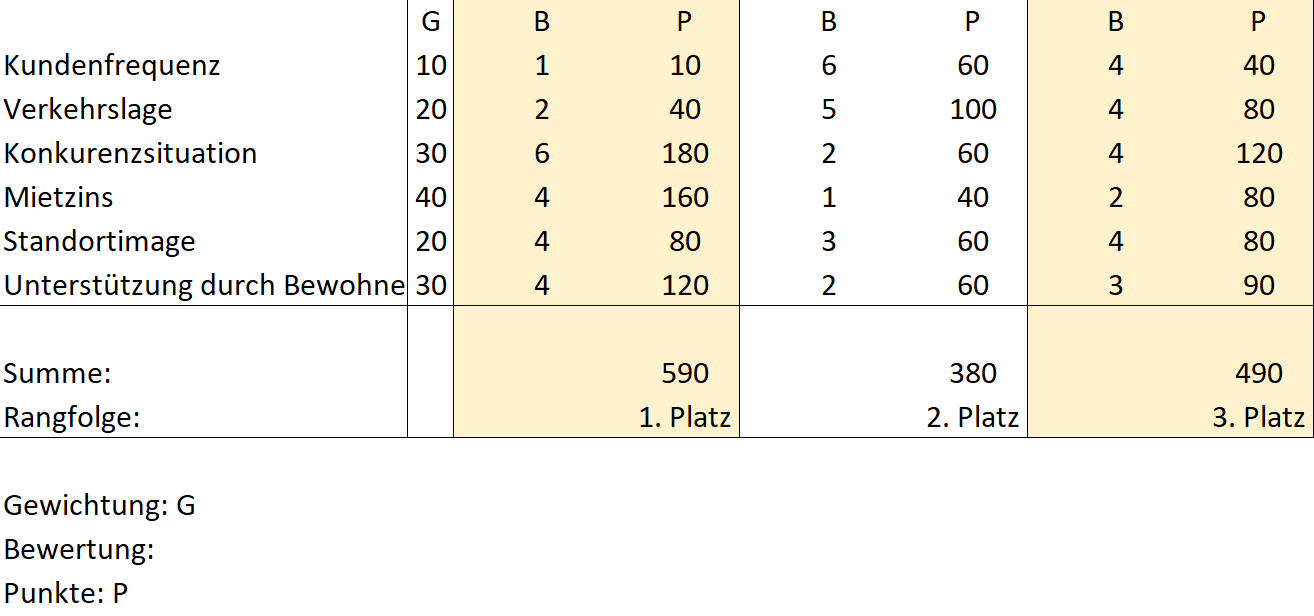
\includegraphics[width=\textwidth]{nutzwerkanalyse}
  \caption{Nutzwerkanalyse}
\end{figure}

\section{Unternehmenskonzept}
\begin{table}[H]
  \begin{tabularx}{\textwidth}{sbbb}
        \hline
         & \textbf{Leistungs-wirtschaftlicher Bereich} & \textbf{Finanz-wirtschaftlicher Bereich} & \textbf{Sozialer \newline Bereich} \\
        \hline
        \textbf{Ziele} & Imageziele, steigende Bekanntschaft & Wirtschaflichkeits-ziele & Gesellschaftsziele, Umweltsziele   \\ \hline
        Beispiel & Wir streben eine Imageverbesserung gegenüber unserer Nachbarschaft um 30\% in den nächsten zwei Jahren an. & Unsere \newline Gesamteinnahmen betragen genug, um in weitere Gadgets zu investieren. & Wir streben eine korrekte Mülltrennung an. \\ \hline
        \textbf{Mittel} & Lärmdämpfung, tolle Angebote, Eintrittsvergünstigung für Dorfbewohner, Werbung. & Durch steigendes Image, wachsende Bekanntschaft und exklusve Musiker möchten wir Gewinne erzielen. & Mit genügend Abfalleimern sowohl in Normal- als auch in Petformat möchten wir eine korrekte Mülltrennung fördern \\ \hline
        Beispiel & Isolierung \newline des Lärmes, Karaokeabende, Vergünstigung des Eintritts um 20\%. & Werbung, eigene Webseite & Abfalleimer ausserhalb und innerhalb, Aschenbecher für Raucher ausserhalb. \\ \hline
        \textbf{Methode} & Werbungs-platzierung, Optimale Lärmisolierung & Erstellung der Website, Wege zur Gewinnmaximierung & Reduzierung von nicht/falsch weggeworfenen Abfällen \\ \hline
        Beispiel & Werbung \newline an öffentlichen Pinnwänden, Zeitungsinserate & Website wird von der Geschäftsführung intern erstellt. & Verwarnung bei Regelverstössen \\ \hline
  \end{tabularx}
  \caption{Unternehmenskonzept}
\end{table}

\end{document}